\section{Results}

To characterize the general selective pressures induced by surveyed environmental conditions, we assessed the prevalence of characteristic multicellular traits among evolved genotypes across replicates.
In the case of an evolutionary transition of individuality, we would expect cells to modulate their own reproductive behavior to prioritize group interests above individual cell interests.
In DISHTINY, cell reproduction inherently destroys an immediate neighbor cell.
As such, we would expect somatic growth to occur primarily at group peripheries in a higher-level individual.
Supplementary Figure \ref{fig:reproduction_surrounded} compares cellular reproduction rates between the interior and exterior of apex-level hereditary groups.
For all treatments, phenotypes with depressed interior cellular reproduction rates dominated across replicates (non-overlapping 95\% CI).
By update 262,144 (about 1,000 cellular generations; see Supplementary Table \ref{tab:systematics}), all four treatment conditions appear to select for some level of reproductive cooperation among cells.

Across replicate evolutionary runs in all four treatments, we also found that resource was transferred among registered kin at a significantly higher mean rate than to unrelated neighbors (non-overlapping 95\% CI).
Genetic programs controlling cells can sense whether any particular neighbor shares a common hereditary group ID.
Thus, selective activation of resource sharing behavior to such neighbors might have evolved, which would provide one possible explanation for this observation.\footnote{
Alternately to the same end, resource sharing behavior could be instead suppressed in the opposite case, when a neighbor holds a different hereditary group ID.
}
However, cells are capable of conditioning behavior on whether a particular neighbor is direct kin (i.e., a parent or child).
To test whether this resource-sharing was solely an artifact of sharing between direct cellular kin, we also assessed mean sharing to registered kin that were not immediate cellular relatives.
Mean sharing between such cells also exceeded sharing among unrelated neighbors (non-overlapping 95\% CI).
Thus, all four treatments appear to select for functional cooperation among wider kin groups.
Supplementary section \ref{sec:resource-sharing} presents these results in detail.

\subsection{Qualitative Life Histories} \label{sec:life-histories}

\begin{figure*}[!htbp]
\begin{center}

\begin{minipage}[b]{\textwidth}
\centering
\begin{minipage}[t]{0.18\textwidth}
\centering
\adjincludegraphics[width=\textwidth, trim={{.5\width} {.33\width} {.17\width} {.38\width}}, clip]{img/lifecycle/naive-paint/seed=1026+title=directional_channel_grayscale_viz+treat=resource-wave__channelsense-yes__nlev-two+update=1048576+_data_hathash_hash=fdd6f7a5210124bd+_script_fullcat_hash=602c0d0c070e9202+_source_hash=53a2252-clean+ext=}
{\footnotesize Update 0}
\end{minipage}
\begin{minipage}[t]{0.18\textwidth}
\centering
\adjincludegraphics[width=\textwidth, trim={{.5\width} {.33\width} {.17\width} {.38\width}}, clip]{img/lifecycle/naive-paint/seed=1026+title=directional_channel_grayscale_viz+treat=resource-wave__channelsense-yes__nlev-two+update=1048704+_data_hathash_hash=fdd6f7a5210124bd+_script_fullcat_hash=602c0d0c070e9202+_source_hash=53a2252-clean+ext=}
{\footnotesize Update 128}
\end{minipage}
\begin{minipage}[t]{0.18\textwidth}
\centering
\adjincludegraphics[width=\textwidth, trim={{.5\width} {.33\width} {.17\width} {.38\width}}, clip]{img/lifecycle/naive-paint/seed=1026+title=directional_channel_grayscale_viz+treat=resource-wave__channelsense-yes__nlev-two+update=1048832+_data_hathash_hash=fdd6f7a5210124bd+_script_fullcat_hash=602c0d0c070e9202+_source_hash=53a2252-clean+ext=}
{\footnotesize Update 256}
\end{minipage}
\begin{minipage}[t]{0.18\textwidth}
\centering
\adjincludegraphics[width=\textwidth, trim={{.5\width} {.33\width} {.17\width} {.38\width}}, clip]{img/lifecycle/naive-paint/seed=1026+title=directional_channel_grayscale_viz+treat=resource-wave__channelsense-yes__nlev-two+update=1048960+_data_hathash_hash=fdd6f7a5210124bd+_script_fullcat_hash=602c0d0c070e9202+_source_hash=53a2252-clean+ext=}
{\footnotesize Update 384}
\end{minipage}
\begin{minipage}[t]{0.18\textwidth}
\centering
\adjincludegraphics[width=\textwidth, trim={{.5\width} {.33\width} {.17\width} {.38\width}}, clip]{img/lifecycle/naive-paint/seed=1026+title=directional_channel_grayscale_viz+treat=resource-wave__channelsense-yes__nlev-two+update=1049088+_data_hathash_hash=fdd6f7a5210124bd+_script_fullcat_hash=602c0d0c070e9202+_source_hash=53a2252-clean+ext=}
{\footnotesize Update 512}
\end{minipage}\\
\begin{minipage}{\textwidth}
\dissertationonly{\footnotesize}
\textbf{(A)}
Naive
(%
animation: \url{https://hopth.ru/x},
in-browser simulation: \url{https://hopth.ru/1}%
).
The offspring group is birthed at the exterior of the parent group.
Parent and offspring groups then compete with each other for space just the same as they do with other groups.
\end{minipage}
% \label{fig:lifecycle-naive}
\end{minipage}

\vspace{3ex}

\begin{minipage}[b]{\textwidth}
\centering
\begin{minipage}[t]{0.18\textwidth}
\centering
\adjincludegraphics[width=\textwidth, trim={{.66\width} {.71\width} {.0\width} {.0\width}}, clip]{img/lifecycle/adjoin-paint/seed=1004+title=directional_channel_grayscale_viz+treat=resource-wave__channelsense-yes__nlev-two+update=1048896+_data_hathash_hash=51fd4923ae7e3bde+_script_fullcat_hash=602c0d0c070e9202+_source_hash=53a2252-clean+ext=}
{\footnotesize Update 0}
\end{minipage}
\begin{minipage}[t]{0.18\textwidth}
\centering
\adjincludegraphics[width=\textwidth, trim={{.66\width} {.71\width} {.0\width} {.0\width}}, clip]{img/lifecycle/adjoin-paint/seed=1004+title=directional_channel_grayscale_viz+treat=resource-wave__channelsense-yes__nlev-two+update=1048928+_data_hathash_hash=51fd4923ae7e3bde+_script_fullcat_hash=602c0d0c070e9202+_source_hash=53a2252-clean+ext=}
{\footnotesize Update 32}
\end{minipage}
\begin{minipage}[t]{0.18\textwidth}
\centering
\adjincludegraphics[width=\textwidth, trim={{.66\width} {.71\width} {.0\width} {.0\width}}, clip]{img/lifecycle/adjoin-paint/seed=1004+title=directional_channel_grayscale_viz+treat=resource-wave__channelsense-yes__nlev-two+update=1048960+_data_hathash_hash=51fd4923ae7e3bde+_script_fullcat_hash=602c0d0c070e9202+_source_hash=53a2252-clean+ext=}
{\footnotesize Update 64}
\end{minipage}
\begin{minipage}[t]{0.18\textwidth}
\centering
\adjincludegraphics[width=\textwidth, trim={{.66\width} {.71\width} {.0\width} {.0\width}}, clip]{img/lifecycle/adjoin-paint/seed=1004+title=directional_channel_grayscale_viz+treat=resource-wave__channelsense-yes__nlev-two+update=1049024+_data_hathash_hash=51fd4923ae7e3bde+_script_fullcat_hash=602c0d0c070e9202+_source_hash=53a2252-clean+ext=}
{\footnotesize Update 128}
\end{minipage}
\begin{minipage}[t]{0.18\textwidth}
\centering
\adjincludegraphics[width=\textwidth, trim={{.66\width} {.71\width} {.0\width} {.0\width}}, clip]{img/lifecycle/adjoin-paint/seed=1004+title=directional_channel_grayscale_viz+treat=resource-wave__channelsense-yes__nlev-two+update=1049408+_data_hathash_hash=51fd4923ae7e3bde+_script_fullcat_hash=602c0d0c070e9202+_source_hash=53a2252-clean+ext=}
{\footnotesize Update 512}
\end{minipage}\\
\begin{minipage}{\textwidth}
\dissertationonly{\footnotesize}
\textbf{(B)} Adjoin
(%
animation: \url{https://hopth.ru/y},
in-browser simulation: \url{https://hopth.ru/2}%
).
The offspring group begins as a single cell at the exterior of the parent group.
Parent and offspring groups then exclusively expend reproductive effort to compete with other groups.
This results in a stable interface between the parent and offspring groups as the offspring group grows over time.
\end{minipage}
% \label{fig:lifecycle-adjoin}
\end{minipage}

\vspace{3ex}

\begin{minipage}[b]{\textwidth}
\centering
\begin{minipage}[t]{0.18\textwidth}
\centering
\adjincludegraphics[width=\textwidth, trim={{.0\width} {.05\width} {.66\width} {.66\width}}, clip]{img/lifecycle/sweep-paint/seed=1023+title=directional_channel_grayscale_viz+treat=resource-wave__channelsense-yes__nlev-two+update=1048648+_data_hathash_hash=519a2d5a19f16020+_script_fullcat_hash=602c0d0c070e9202+_source_hash=53a2252-clean+ext=}
{\footnotesize Update 0}
\end{minipage}
\begin{minipage}[t]{0.18\textwidth}
\centering
\adjincludegraphics[width=\textwidth, trim={{.0\width} {.05\width} {.66\width} {.66\width}}, clip]{img/lifecycle/sweep-paint/seed=1023+title=directional_channel_grayscale_viz+treat=resource-wave__channelsense-yes__nlev-two+update=1048720+_data_hathash_hash=519a2d5a19f16020+_script_fullcat_hash=602c0d0c070e9202+_source_hash=53a2252-clean+ext=}
{\footnotesize Update 72}
\end{minipage}
\begin{minipage}[t]{0.18\textwidth}
\centering
\adjincludegraphics[width=\textwidth, trim={{.0\width} {.05\width} {.66\width} {.66\width}}, clip]{img/lifecycle/sweep-paint/seed=1023+title=directional_channel_grayscale_viz+treat=resource-wave__channelsense-yes__nlev-two+update=1048792+_data_hathash_hash=519a2d5a19f16020+_script_fullcat_hash=602c0d0c070e9202+_source_hash=53a2252-clean+ext=}
{\footnotesize Update 144}
\end{minipage}
\begin{minipage}[t]{0.18\textwidth}
\centering
\adjincludegraphics[width=\textwidth, trim={{.0\width} {.05\width} {.66\width} {.66\width}}, clip]{img/lifecycle/sweep-paint/seed=1023+title=directional_channel_grayscale_viz+treat=resource-wave__channelsense-yes__nlev-two+update=1048864+_data_hathash_hash=519a2d5a19f16020+_script_fullcat_hash=602c0d0c070e9202+_source_hash=53a2252-clean+ext=}
{\footnotesize Update 216}
\end{minipage}
\begin{minipage}[t]{0.18\textwidth}
\centering
\adjincludegraphics[width=\textwidth, trim={{.0\width} {.05\width} {.66\width} {.66\width}}, clip]{img/lifecycle/sweep-paint/seed=1023+title=directional_channel_grayscale_viz+treat=resource-wave__channelsense-yes__nlev-two+update=1048936+_data_hathash_hash=519a2d5a19f16020+_script_fullcat_hash=602c0d0c070e9202+_source_hash=53a2252-clean+ext=}
{\footnotesize Update 288}
\end{minipage}\\
\begin{minipage}{\textwidth}
\dissertationonly{\footnotesize}
\textbf{(C)} Sweep
(%
animation: \url{https://hopth.ru/z},
in-browser simulation: \url{https://hopth.ru/3}%
).
The offspring group begins as a single cell at the exterior of the parent group.
The offspring group then grows rapidly into the parent group, resulting in a near-complete transfer of simulation space into the offspring group.
Multiple offspring groups may simultaneously grow over the parent, as is the case here.
\end{minipage}
% \label{fig:lifecycle-sweep}
\end{minipage}

\vspace{3ex}

\begin{minipage}[b]{\textwidth}
\centering
\begin{minipage}[t]{0.18\textwidth}
\centering
\adjincludegraphics[width=\textwidth, trim={{.0\width} {.71\width} {.66\width} {.0\width}}, clip]{img/lifecycle/burst-paint/seed=1034+title=directional_channel_grayscale_viz+treat=resource-wave__channelsense-yes__nlev-two+update=1048648+_data_hathash_hash=ca8ad21d3b30b939+_script_fullcat_hash=602c0d0c070e9202+_source_hash=53a2252-clean+ext=}
{\footnotesize Update 0}
\end{minipage}
\begin{minipage}[t]{0.18\textwidth}
\centering
\adjincludegraphics[width=\textwidth, trim={{.0\width} {.71\width} {.66\width} {.0\width}}, clip]{img/lifecycle/burst-paint/seed=1034+title=directional_channel_grayscale_viz+treat=resource-wave__channelsense-yes__nlev-two+update=1048744+_data_hathash_hash=ca8ad21d3b30b939+_script_fullcat_hash=602c0d0c070e9202+_source_hash=53a2252-clean+ext=}
{\footnotesize Update 96}
\end{minipage}
\begin{minipage}[t]{0.18\textwidth}
\centering
\adjincludegraphics[width=\textwidth, trim={{.0\width} {.71\width} {.66\width} {.0\width}}, clip]{img/lifecycle/burst-paint/seed=1034+title=directional_channel_grayscale_viz+treat=resource-wave__channelsense-yes__nlev-two+update=1048840+_data_hathash_hash=ca8ad21d3b30b939+_script_fullcat_hash=602c0d0c070e9202+_source_hash=53a2252-clean+ext=}
{\footnotesize Update 192}
\end{minipage}
\begin{minipage}[t]{0.18\textwidth}
\centering
\adjincludegraphics[width=\textwidth, trim={{.0\width} {.71\width} {.66\width} {.0\width}}, clip]{img/lifecycle/burst-paint/seed=1034+title=directional_channel_grayscale_viz+treat=resource-wave__channelsense-yes__nlev-two+update=1048936+_data_hathash_hash=ca8ad21d3b30b939+_script_fullcat_hash=602c0d0c070e9202+_source_hash=53a2252-clean+ext=}
{\footnotesize Update 288}
\end{minipage}
\begin{minipage}[t]{0.18\textwidth}
\centering
\adjincludegraphics[width=\textwidth, trim={{.0\width} {.71\width} {.66\width} {.0\width}}, clip]{img/lifecycle/burst-paint/seed=1034+title=directional_channel_grayscale_viz+treat=resource-wave__channelsense-yes__nlev-two+update=1049032+_data_hathash_hash=ca8ad21d3b30b939+_script_fullcat_hash=602c0d0c070e9202+_source_hash=53a2252-clean+ext=}
{\footnotesize Update 384}
\end{minipage}\\
\begin{minipage}{\textwidth}
\dissertationonly{\footnotesize}
\textbf{(D)} Burst
(%
animation: \url{https://hopth.ru/0},
in-browser simulation: \url{https://hopth.ru/4}%
).
The offspring group begins as a single cell at the interior of the parent group.
Over time, the offspring group grows over the parent group from the inside out.
Multiple offspring groups may develop simultaneously, as is the case here.
\end{minipage}
% \label{fig:lifecycle-burst}
\end{minipage}

\caption{
Time lapse examples of qualitative life histories evolved under the Nested-Wave treatment.
From left to right within each row, frames depict the progression of simulation state within a subset of the simulation grid.
L1 hereditary groups are by differentiated by grayscale tone and separated by solid black borders.
L0 hereditary groups are by separated by dashed gray borders.
In each example, the focal parent L1 group is colored purple and the focal offspring group orange.
}
\label{fig:lifecycle}
\end{center}
\end{figure*}


Although cooperative cell-level phenotypes were common among evolved hereditary groups, across replicates functional and reproductive cooperation arose via diverse qualitative life histories.
To provide a general sense for the types of life histories we observed in this system, Figure \ref{fig:lifecycle} shows time lapses of representative multicellular groups evolved in different replicates.
Figure \ref{fig:lifecycle}\textbf{(A)} depicts an example of a naive life history in which --- beyond the cellular progenitor of a propagule group --- the parent and propagule groups exhibit no special cooperative relationship.
In Figure \ref{fig:lifecycle}\textbf{(B)}, propagules repeatedly bud off of parent groups to yield a larger network of persistent parent-child cooperators.
In Figure \ref{fig:lifecycle}\textbf{(C)}, propagules are generated at the extremities of parent groups and then rapidly replace most or all of the parent group.
Finally, in Figure \ref{fig:lifecycle}\textbf{(D)}, propagules are generated at the interior of a parent group and replace it from the inside out.

To better understand the multicellular strategies that evolved in this system, we investigated the mechanisms and adaptiveness of notable phenotypes that evolved in several individual evolutionary replicates.
In the following sections, we present these investigations as a series of case studies.

%Section \ref{sec:gene-regulation} reports a particular group-replication strategy in which propagule groups are seeded within the soma, destroying the parent as they mature.


\subsection{Case Study: Burst Lifecycle} \label{sec:gene-regulation}

\begin{figure}[!htbp]
\begin{center}

\begin{minipage}[t]{0.5\linewidth}

% \begin{minipage}[b]{\linewidth}
% \begin{center}

% \begin{minipage}[t]{0.18\linewidth}
% \centering
% \vspace{0pt} % for alignment
% \adjincludegraphics[width=\textwidth, trim={{.0\width} {.77\width} {.79\width} {.02\width}}, clip]{img/lifecycle/burst-paint/seed=1034+title=directional_channel_grayscale_viz+treat=resource-wave__channelsense-yes__nlev-two+update=1048648+_data_hathash_hash=ca8ad21d3b30b939+_script_fullcat_hash=602c0d0c070e9202+_source_hash=53a2252-clean+ext=}
% \footnotesize Update 0
% \end{minipage}
% \begin{minipage}[t]{0.18\linewidth}
% \centering
% \vspace{0pt} % for alignment
% \adjincludegraphics[width=\textwidth, trim={{.0\width} {.77\width} {.79\width} {.02\width}}, clip]{img/lifecycle/burst-paint/seed=1034+title=directional_channel_grayscale_viz+treat=resource-wave__channelsense-yes__nlev-two+update=1048744+_data_hathash_hash=ca8ad21d3b30b939+_script_fullcat_hash=602c0d0c070e9202+_source_hash=53a2252-clean+ext=}
% \footnotesize 96
% \end{minipage}
% \begin{minipage}[t]{0.18\linewidth}
% \centering
% \vspace{0pt} % for alignment
% \adjincludegraphics[width=\textwidth, trim={{.0\width} {.77\width} {.79\width} {.02\width}}, clip]{img/lifecycle/burst-paint/seed=1034+title=directional_channel_grayscale_viz+treat=resource-wave__channelsense-yes__nlev-two+update=1048840+_data_hathash_hash=ca8ad21d3b30b939+_script_fullcat_hash=602c0d0c070e9202+_source_hash=53a2252-clean+ext=}
% \footnotesize 192
% \end{minipage}
% \begin{minipage}[t]{0.18\linewidth}
% \centering
% \vspace{0pt} % for alignment
% \adjincludegraphics[width=\textwidth, trim={{.0\width} {.77\width} {.79\width} {.02\width}}, clip]{img/lifecycle/burst-paint/seed=1034+title=directional_channel_grayscale_viz+treat=resource-wave__channelsense-yes__nlev-two+update=1048936+_data_hathash_hash=ca8ad21d3b30b939+_script_fullcat_hash=602c0d0c070e9202+_source_hash=53a2252-clean+ext=}
% \footnotesize 288
% \end{minipage}
% \begin{minipage}[t]{0.18\linewidth}
% \centering
% \vspace{0pt} % for alignment
% \adjincludegraphics[width=\textwidth, trim={{.0\width} {.77\width} {.79\width} {.02\width}}, clip]{img/lifecycle/burst-paint/seed=1034+title=directional_channel_grayscale_viz+treat=resource-wave__channelsense-yes__nlev-two+update=1049032+_data_hathash_hash=ca8ad21d3b30b939+_script_fullcat_hash=602c0d0c070e9202+_source_hash=53a2252-clean+ext=}
% \footnotesize 384
% \end{minipage}
% \caption{Wild type timelapse}
% \label{fig:wt_timelapse}
% \end{center}
% \end{minipage}

% \vspace{2ex}

\begin{minipage}[b]{\linewidth}
\begin{center}

\begin{minipage}[t]{0.30\linewidth}
\centering
\vspace{0pt} % for alignment
% adapted from https://tex.stackexchange.com/a/186476
\begin{tikzpicture}
\node[anchor=south west,inner sep=0] (image) at (0,0) { \adjincludegraphics[width=\linewidth, trim={{.25\width} {.20\width} {.5\width} {.55\width}}, clip]{img/knockout/interior_propagule/wildtype/retouched3_seed=1+title=directional_regulator_viz+treat=resource-wave__channelsense-yes__nlev-two+update=8188+_data_hathash_hash=8b493febd79aad1f+_script_fullcat_hash=90718bb0c6ec4dbd+_source_hash=53a2252-clean+ext=}
};
\begin{scope}[x={(image.south east)},y={(image.north west)}]
  \draw [ultra thick,-{stealth[scale=1.25]}, white] (0.35,0.59) -- ++(0.06,-0.06);
  \draw [ultra thick, -{stealth[scale=1.25]}, white] (0.01,0.39) -- ++(0.06,-0.06);
  \draw [ultra thick, -{stealth[scale=1.25]}, white] (0.68,0.39) -- ++(0.06,-0.06);
  \draw [ultra thick, -{stealth[scale=1.25]}, white] (0.62,0.32) -- ++(0.06,-0.06);
  \draw [-stealth, red] (0.35,0.59) -- ++(0.05,-0.05);
  \draw [-stealth, red] (0.01,0.39) -- ++(0.05,-0.05);
  \draw [-stealth, red] (0.68,0.39) -- ++(0.05,-0.05);
  \draw [-stealth, red] (0.62,0.32) -- ++(0.05,-0.05);
\end{scope}
\end{tikzpicture}
\footnotesize Wild type
\end{minipage}
\begin{minipage}[t]{0.30\linewidth}
\centering
\vspace{0pt} % for alignment
\adjincludegraphics[width=\linewidth, trim={{.5\width} {.5\width} {.25\width} {.25\width}}, clip]{img/knockout/interior_propagule/propaguleknockout/retouched2_seed=1+title=directional_regulator_viz+treat=resource-wave__channelsense-yes__nlev-two+update=8188+_data_hathash_hash=2b6711db47fb5887+_script_fullcat_hash=90718bb0c6ec4dbd+_source_hash=53a2252-clean+ext=}
\footnotesize Propagule knockout
\end{minipage}
\begin{minipage}[t]{0.30\linewidth}
\centering
\vspace{0pt} % for alignment
\adjincludegraphics[width=\linewidth, trim={{.5\width} {.5\width} {.25\width} {.25\width}}, clip]{img/knockout/interior_propagule/regulationknockout/retouched_seed=1+title=directional_regulator_viz+treat=resource-wave__channelsense-yes__nlev-two+update=8188+_data_hathash_hash=11ab5cdd47ed18c7+_script_fullcat_hash=90718bb0c6ec4dbd+_source_hash=53a2252-clean+ext=}
\footnotesize Regulation knockout
\end{minipage}

{\textbf{(A)} Regulation visualizations}
% \label{fig:regulation_visualizations}

\end{center}
\end{minipage}

\begin{minipage}[t]{\linewidth}
\centering
\vspace{0pt} % for alignment
\begin{minipage}[b]{\linewidth}
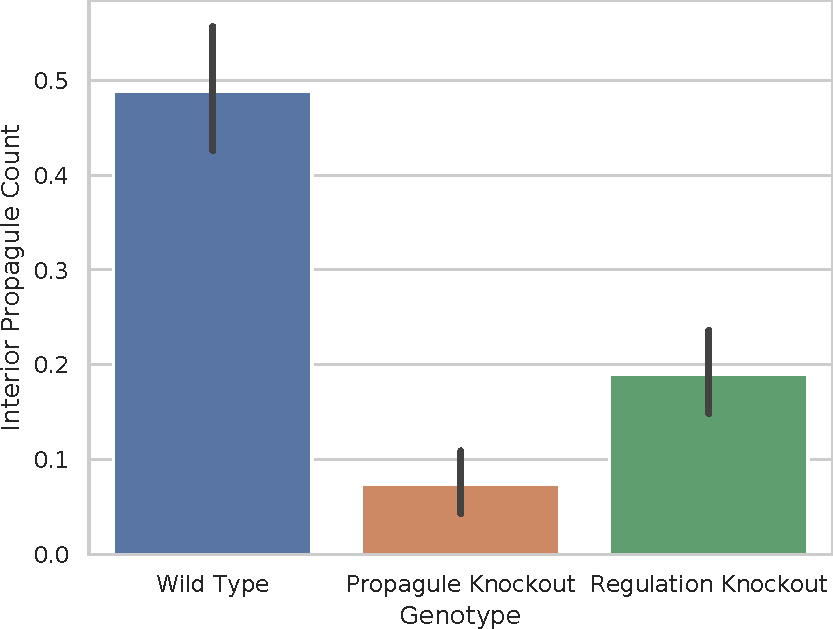
\includegraphics[width=\linewidth]{img/knockout/interior_propagule/title=interior_propagules+_data_hathash_hash=bb0fa6254f1b7398+_script_fullcat_hash=f738b363bea8c98a+_source_hash=53a2252-clean+ext=}
{\textbf{(B)} Interior propagule rate by genotype}
% \label{fig:interior_propagule_rate}
\end{minipage}
\end{minipage}%
\hspace*{\fill}

\end{minipage}

\caption{
Analysis of a wild type strain exhibiting a ``burst'' lifecycle evolved under the ``Nested-Wave'' treatment exhibiting interior propagule generation.
% Figure \ref{fig:wt_timelapse} traces the wild type life history.
% L1 hereditary groups are by differentiated by grayscale tone and separated by solid black borders.
% L0 hereditary groups are by separated by gray borders.
% In each example, the focal parent L1 hereditary group is colored purple and the focal offspring group orange.
Subfigure \textbf{(A)} compares gene regulation between analyzed strains.
Group layouts are overlaid via borders between cells.
Black borders divide L1 groups and white borders divide L0 groups.
Borders between L1 groups are underlined in red for greater visibility.
state for each cell's four directional SignalGP instances.
Within these group layouts, regulation state for each cell's four directional SignalGP instances is color coded using a PCA mapping from regulatory state to three-dimensional RGB coordinates.
(The PCA mapping is calculated uniquely for each L1 hereditary group.)
Within a L1 hereditary group, color similarity among tile quarters indicates that the corresponding SignalGP instances exhibit similar regulatory state.
In the case of identical regulatory state (here, due to the absence of genetic regulation in a knockout strain) this color coding appears gray.
Wild type interior propagules are annotated with red arrows.
Subfigure \textbf{(B)} compares the mean number of interior propagules observed per L1 hereditary group.
Error bars indicate 95\% confidence.
View an animation of wild type gene regulation at \url{https://hopth.ru/t}.
View the wild type strain in a live in-browser simulation at \url{https://hopth.ru/g}.
}
\label{fig:ko-interior_propagule}
\end{center}
\end{figure}


%This wild type strain exhibits an irregular, but somewhat concentric, spatial pattern of gene regulation illustrated in Figure \ref{fig:ko-interior_propagule}\textbf{(A)}.
%In time-series animation, linked in the figure caption, gene regulation appears to fluctuate dynamically.

We wondered how the strain exhibiting the ``burst'' lifecycle in Figure \ref{fig:lifecycle}\textbf{(D)} determined when and where to originate its propagules.
To assess whether gene regulation instructions played a role in this process, we prepared two knockout strains.
In the first, gene regulation instructions were replaced with no-operation (Nop) instructions (so that gene regulation state would remain baseline).
In the second, the reproduction instructions to spawn a propagule were replaced with Nop instructions.
Figure \ref{fig:ko-interior_propagule}\textbf{(A)} depicts the gene regulation phenotypes of these strains.

Figure \ref{fig:ko-interior_propagule}\textbf{(B)} compares interior propagule generation between the strains, confirming the direct mechanistic role of gene regulation in promoting interior propagule generation (non-overlapping 95\% CI).

In head-to-head match-ups, the wild type strain outcompetes both the regulation-knockout ($20/20$; $p < 0.001$; two-tailed Binomial test) and the propagule-knockout strains
($20/20$; $p < 0.001$; two-tailed Binomial test).
The deficiency of the propagule-knockout strain confirms the adaptive role of interior propagule generation.
Likewise, the deficiency of the regulation-knockout strain affirms the adaptive role of gene regulation in the focal wild type strain.

\subsection{Case Study: Cell-cell Messaging} \label{sec:cell-cell-messaging}

\begin{figure}[!htbp]
\begin{center}

\begin{minipage}[t]{0.5\linewidth}

\begin{minipage}[t]{\linewidth}
\hspace*{\fill}%
\begin{minipage}[t]{0.05\linewidth}
\vspace{0pt} % for alignment
\rotatebox{90}{Messaging}%
\end{minipage}%
\hfill
\begin{minipage}[t]{0.45\linewidth}
\centering
\vspace{0pt} % for alignment
\adjincludegraphics[width=\textwidth, trim={{.0\width} {.0\width} {.5\width} {.5\width}}, clip]{img/knockout/intermessaging-sharing/wildtype/seed=1+title=directional_messaging_viz+treat=resource-wave__channelsense-yes__nlev-onebig+update=7172+_data_hathash_hash=f9e2a8ff33bf7745+_script_fullcat_hash=6b7e0389992dd616+_source_hash=53a2252-clean+ext=}%
\end{minipage}%
\hfill
\begin{minipage}[t]{0.45\linewidth}
\centering
\vspace{0pt} % for alignment
\adjincludegraphics[width=\textwidth, trim={{.0\width} {.0\width} {.5\width} {.5\width}}, clip]{img/knockout/intermessaging-sharing/knockout/seed=1+title=directional_messaging_viz+treat=resource-wave__channelsense-yes__nlev-onebig+update=7172+_data_hathash_hash=ffdeb1c77dd012e1+_script_fullcat_hash=6b7e0389992dd616+_source_hash=53a2252-clean+ext=}%
\end{minipage}%
\hspace*{\fill}

\hspace*{\fill}%
\begin{minipage}[t]{0.05\linewidth}
\vspace{0pt} % for alignment
\rotatebox{90}{Resource Sharing}%
\end{minipage}%
\hfill
\begin{minipage}[t]{0.45\linewidth}
\centering
\vspace{0pt} % for alignment
\adjincludegraphics[width=\textwidth, trim={{.0\width} {.0\width} {.5\width} {.5\width}}, clip]{img/knockout/intermessaging-sharing/wildtype/seed=1+title=directional_sharing_viz+treat=resource-wave__channelsense-yes__nlev-onebig+update=7172+_data_hathash_hash=f9e2a8ff33bf7745+_script_fullcat_hash=3a1e851383e0ffd4+_source_hash=53a2252-clean+ext=}%
\end{minipage}%
\hfill
\begin{minipage}[t]{0.45\linewidth}
\centering
\vspace{0pt} % for alignment
\adjincludegraphics[width=\textwidth, trim={{.0\width} {.0\width} {.5\width} {.5\width}}, clip]{img/knockout/intermessaging-sharing/knockout/seed=1+title=directional_sharing_viz+treat=resource-wave__channelsense-yes__nlev-onebig+update=7172+_data_hathash_hash=ffdeb1c77dd012e1+_script_fullcat_hash=3a1e851383e0ffd4+_source_hash=53a2252-clean+ext=}%
\end{minipage}%
\hspace*{\fill}

\hspace*{\fill}%
\begin{minipage}[t]{0.05\linewidth}
\vspace{0pt} % for alignment
\rotatebox{90}{Resource Stockpile}%
\end{minipage}%
\hfill
\begin{minipage}[t]{0.45\linewidth}
\centering
\vspace{0pt} % for alignment
\adjincludegraphics[width=\textwidth, trim={{.0\width} {.0\width} {.5\width} {.5\width}}, clip]{img/knockout/intermessaging-sharing/wildtype/seed=1+title=stockpile_viz+treat=resource-wave__channelsense-yes__nlev-onebig+update=7172+_data_hathash_hash=f9e2a8ff33bf7745+_script_fullcat_hash=4c8152cbf92e0da6+_source_hash=53a2252-clean+ext=}%
\end{minipage}%
\hfill
\begin{minipage}[t]{0.45\linewidth}
\centering
\vspace{0pt} % for alignment
\adjincludegraphics[width=\textwidth, trim={{.0\width} {.0\width} {.5\width} {.5\width}}, clip]{img/knockout/intermessaging-sharing/knockout/seed=1+title=stockpile_viz+treat=resource-wave__channelsense-yes__nlev-onebig+update=7172+_data_hathash_hash=ffdeb1c77dd012e1+_script_fullcat_hash=4c8152cbf92e0da6+_source_hash=53a2252-clean+ext=}%
\end{minipage}%
\hspace*{\fill}

\vspace{1.0ex}

\hspace*{\fill}%
\begin{minipage}[t]{0.05\linewidth}
\vspace{0pt} % for alignment
\end{minipage}%
\hfill
\begin{minipage}[t]{0.45\linewidth}
\centering
\vspace{0pt} % for alignment
Wild Type
\end{minipage}%
\hfill
\begin{minipage}[t]{0.45\linewidth}
\centering
\vspace{0pt} % for alignment
Messaging Knockout
\end{minipage}%
\hspace*{\fill}

\vspace{1.0ex}

% \begin{minipage}{\linewidth}
%   \caption{Phenotype visualizations}
%   \label{fig:intermessaging-sharing-phen}
% \end{minipage}

\end{minipage}%
% \begin{minipage}[t]{\linewidth}
%
% \hspace*{\fill}%
% \begin{minipage}[t]{\textwidth}
% \centering
% \vspace{0pt} % for alignment
% \begin{minipage}[b]{\textwidth}
% \includegraphics[width=\textwidth]{img/knockout/intermessaging-sharing/title=sharingdirection+_data_hathash_hash=59f6520a17fb3ad8+_script_fullcat_hash=97aad8dce5e50084+_source_hash=53a2252-clean+ext=}%
% \caption{Net sharing direction variance}
% \label{fig:intermessaging-sharing-direction}
% \end{minipage}
% \end{minipage}%
% \hfill
% \begin{minipage}[t]{\textwidth}
% \centering
% \vspace{0pt} % for alignment
% \begin{minipage}[b]{\textwidth}
% 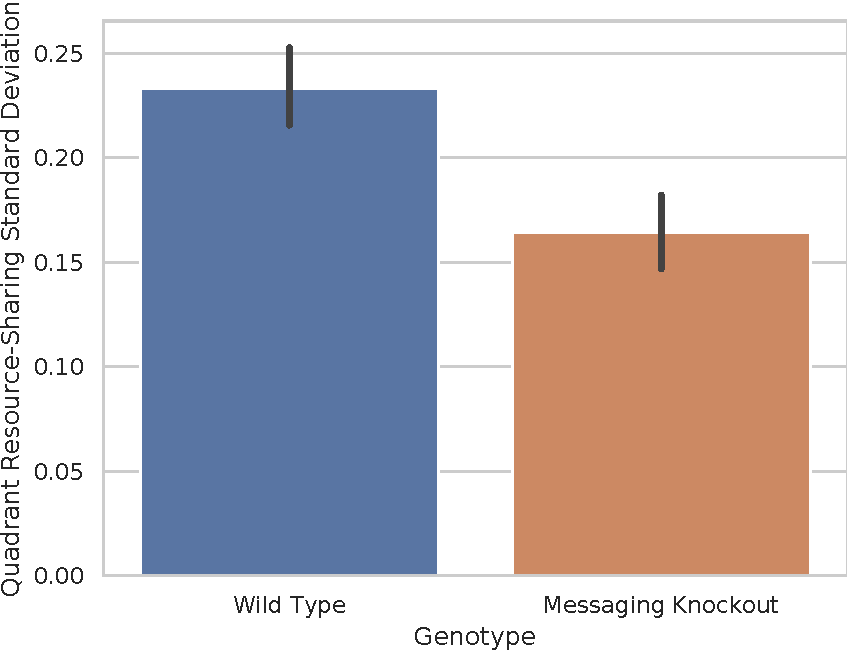
\includegraphics[width=\textwidth]{img/knockout/intermessaging-sharing/title=sharingquadrant+_data_hathash_hash=586f3c805332c323+_script_fullcat_hash=6e8aa37a96d9d7a9+_source_hash=53a2252-clean+ext=}%
% \caption{Net sharing localization variance}
% \label{fig:intermessaging-sharing-quadrant}
% \end{minipage}
% \end{minipage}%
% \hfill
% \begin{minipage}[t]{\textwidth}
% \centering
% \vspace{0pt} % for alignment
% \begin{minipage}[b]{\textwidth}
% \includegraphics[width=\textwidth]{img/knockout/intermessaging-sharing/title=fractionresevoir+_data_hathash_hash=7ce9af7e8fe0699b+_script_fullcat_hash=da31ee3af7ae0208+_source_hash=53a2252-clean+ext=}%
% \caption{Fraction of cells with enough resource to reproduce}
% \label{fig:intermessaging-sharing-resevoir}
% \end{minipage}
% \end{minipage}%
% \hspace*{\fill}
% \end{minipage}

\end{minipage}

\caption{
Visualization of phenotypic traits of a wild type strain evolved under the ``Flat-Wave'' treatment and corresponding intercell messaging knockout strain.
For these visualizations, group layouts are overlaid via borders between cells.
Black borders divide L0 hereditary groups.
In the messaging visualization, color coding represents the volume of incoming messages.
White represents no incoming messages and the magenta to blue gradient runs from one incoming message to the maximum observed incoming message traffic.
Unlike the wild type strain, as expected the messaging knockout strain exhibits no messaging activity.
In the resource sharing visualization, color coding represents the amount of incoming resource.
White represents no incoming resource and the magenta to blue gradient runs from the minimum to the maximum observed incoming incoming resource.
The wild type strain exhibits much more sparse resource sharing than the messaging knockout strain.
In the resource stockpile visualization, white represents zero-resource stockpiles, blue represents stockpiles with just under enough resource to reproduce, green represents stockpiles with enough resource to reproduce, and yellow represents more than enough resource to reproduce.
The wild type groups contain more cells with rich resource stockpiles (green and yellow) than the messaging knockout strain.
View an animation of the wild type strain at \url{https://hopth.ru/p}.
View the wild type strain in a live in-browser simulation at \url{https://hopth.ru/e}.
% minipages \ref{fig:intermessaging-sharing-direction}, \ref{fig:intermessaging-sharing-quadrant}, \ref{fig:intermessaging-sharing-resevoir} quantify knockout effects on various phenotypic traits.
% Error bars indicate 95\% confidence.
}
\label{fig:ko-intermessaging-sharing}
\end{center}
\end{figure}


We discovered adaptive cell-cell messaging in two evolved strains.
Here, we discuss a strain evolved under the Flat-Wave treatment where cell-cell messaging disrupts directional and spatial uniformity of resource sharing.
Supplementary Section \ref{sec:intergroup} overviews an evolved strain where cell-cell messaging appears to intensify expression of a contextual tit-for-tat policy between hereditary groups.

Figure \ref{fig:ko-intermessaging-sharing} depicts the cell-cell messaging, resource sharing, and resource stockpile phenotypes of the wild type strain side-by-side with corresponding phenotypes of a cell-cell messaging knockout strain.
In the wild type strain, cell-cell messaging emanates from irregular collection of cells --- in some regions, grid-like and in others more sparse --- broadcasting to all neighboring cells.
Resource sharing appears more widespread in the knockout strain than in the wild type.
However, messaging's effects suppressing resource sharing is neither spatially nor directionally homogeneous.
Relative to the knockout strain, cell-cell messaging increases variance in cardinal directionality of net resource sharing
(%
WT: mean 0.28, S.D. 0.07, $n=54$; % 2020/01-06-ll.md
KO: mean 0.17, S.D. 0.07, $n=69$; % 2020/01-06-ll.md
%Figure \ref{fig:intermessaging-sharing-direction};
$p < 0.001$, bootstrap test%
).
Cell-cell messaging also increases variance of resource sharing density with respect to spatial quadrants demarcated by the hereditary group's spatial centroid
(%
WT: mean 0.23, S.D. 0.07, $n=52$; % 2020/01-06-ll.md
KO: mean 0.16, S.D. 0.08, $n=68$; % 2020/01-06-ll.md
%Figure \ref{fig:intermessaging-sharing-quadrant};
$p < 0.001$, bootstrap test% 2020/01-06-ll.md
).
We used competition experiments to confirm the fitness advantage both of cell-cell messaging ($20/20$; $p < 0.001$; two-tailed Binomial test) and (using a separate knockout strain) resource sharing ($20/20$; $p < 0.001$; two-tailed Binomial test).
The fitness advantage of irregularized sharing might stem from a corresponding increase in the fraction of cells with enough resource to reproduce stockpiled
(%
WT: mean 0.18, S.D. 0.11, $n=54$; % 2020/01-06-ll.md
KO: mean 0.06, S.D. 0.08, $n=69$; % 2020/01-06-ll.md
$p < 0.001$, bootstrap test% 2020/01-06-ll.md
).

\subsection{Case Study: Gradient-conditioned Cell Behavior} \label{sec:gradient-conditioned-behavior}

\begin{figure}[!htbp]
\begin{center}

\centering

\hspace*{\fill}%
\begin{minipage}[t]{0.05\columnwidth}
\vspace{0pt} % for alignment
\rotatebox{90}{Resource Stockpile}%
\end{minipage}%
\hfill
\begin{minipage}[t]{0.45\columnwidth}
\centering
\vspace{0pt} % for alignment
\adjincludegraphics[width=\textwidth, trim={{.0\width} {.0\width} {.5\width} {.5\width}}, clip]{img/knockout/stockpiletrigger-sharing/wildtype/seed=1+title=stockpile_viz+treat=resource-wave__channelsense-yes__nlev-two+update=7172+_data_hathash_hash=d856da4ae5863122+_script_fullcat_hash=4c8152cbf92e0da6+_source_hash=53a2252-clean+ext=}%
\end{minipage}%
\hfill
\begin{minipage}[t]{0.45\columnwidth}
\centering
\vspace{0pt} % for alignment
\adjincludegraphics[width=\textwidth, trim={{.0\width} {.0\width} {.5\width} {.5\width}}, clip]{img/knockout/stockpiletrigger-sharing/knockout/seed=1+title=stockpile_viz+treat=resource-wave__channelsense-yes__nlev-two+update=7172+_data_hathash_hash=6ab6ade50c5344bc+_script_fullcat_hash=4c8152cbf92e0da6+_source_hash=53a2252-clean+ext=}%
\end{minipage}%
\hspace*{\fill}


\hspace*{\fill}%
\begin{minipage}[t]{0.05\columnwidth}
\vspace{0pt} % for alignment
\rotatebox{90}{Resource Sharing}%
\end{minipage}%
\hfill
\begin{minipage}[t]{0.45\columnwidth}
\centering
\vspace{0pt} % for alignment
\adjincludegraphics[width=\textwidth, trim={{.0\width} {.0\width} {.5\width} {.5\width}}, clip]{img/knockout/stockpiletrigger-sharing/wildtype/seed=1+title=directional_sharing_viz+treat=resource-wave__channelsense-yes__nlev-two+update=7172+_data_hathash_hash=d856da4ae5863122+_script_fullcat_hash=3a1e851383e0ffd4+_source_hash=53a2252-clean+ext=}%
\end{minipage}%
\hfill
\begin{minipage}[t]{0.45\columnwidth}
\centering
\vspace{0pt} % for alignment
\adjincludegraphics[width=\textwidth, trim={{.0\width} {.0\width} {.5\width} {.5\width}}, clip]{img/knockout/stockpiletrigger-sharing/knockout/seed=1+title=directional_sharing_viz+treat=resource-wave__channelsense-yes__nlev-two+update=7172+_data_hathash_hash=6ab6ade50c5344bc+_script_fullcat_hash=3a1e851383e0ffd4+_source_hash=53a2252-clean+ext=}%
\end{minipage}%
\hspace*{\fill}

\vspace{1.0ex}

\hspace*{\fill}%
\begin{minipage}[t]{0.05\columnwidth}
\vspace{0pt} % for alignment
\end{minipage}%
\hfill
\begin{minipage}[t]{0.45\columnwidth}
\centering
\vspace{0pt} % for alignment
Wild Type
\end{minipage}%
\hfill
\begin{minipage}[t]{0.45\columnwidth}
\centering
\vspace{0pt} % for alignment
Relative Stockpile Sensing Knockout
\end{minipage}%
\hspace*{\fill}

\vspace{1.0ex}

\caption{
Visualization of phenotypic traits of a wild type strain evolved under the ``Nested-Wave'' treatment and corresponding resource-sensing knockout strain.
For these visualizations, group layouts are overlaid via borders between cells.
Black borders divide L1 hereditary groups and dashed gray borders divide L0 hereditary groups.
In the resource stockpile visualization, white represents zero-resource stockpiles, blue represents stockpiles with just under enough resource to reproduce, green represents stockpiles with enough resource to reproduce, and yellow represents more than enough resource to reproduce.
The wild type groups contain more cells with rich resource stockpiles (green and yellow) than the knockout strain.
In the resource-sharing visualization, white represents no incoming resource and the magenta to blue gradient runs from the minimum to the maximum observed amount of incoming shared resource.
The wild type strain exhibits less resource sharing than the knockout strain.
View an animation of the wild type strain at \url{https://hopth.ru/s}.
View the wild type strain in a live in-browser simulation at \url{https://hopth.ru/h}.
}
\label{fig:ko-stockpiletrigger-sharing}
\end{center}
\end{figure}


To further assess how multicellular groups process and employ spatial and directional information, we investigated whether successful multicellular strategies evolved where cells condition their behavior based on the resource concentration gradient within a multicellular group.
We discovered a strain that employs a dynamic strategy where cells condition their own resource-sharing behavior based on the relative abundance of their own resource stockpiles compared to their neighbors.
This strain appears to use this information to selectively suppress resource sharing.
This strain's wild type outcompeted a variant where cells' capacity to assess relative richness of neighboring resource stockpiles was knocked out ($20/20$; $p < 0.001$; two-tailed Binomial test).
Figure \ref{fig:ko-stockpiletrigger-sharing} contrasts the wild type resource-sharing phenotype with the more sparse knockout resource-sharing phenotype.

This result raises the question of whether more sophisticated morphological patterning might evolve within the experimental system.
Next, in Section \ref{sec:morphology}, we examine a strain that exhibited striking genetically driven morphological patterning of hereditary groups.

\subsection{Case Study: Morphology} \label{sec:morphology}

\begin{figure}[!htbp]
\begin{center}

\begin{minipage}[t]{\linewidth}

\hspace*{\fill}%
\begin{minipage}[t]{0.22\linewidth}
\centering
\vspace{0pt} % for alignment
\begin{minipage}[b]{\textwidth}
\adjincludegraphics[width=\textwidth, trim={{.0\width} {.0\width} {.5\width} {.5\width}}, clip]{img/knockout/morphology/wildtype/seed=1+title=channel_viz+treat=resource-even__channelsense-yes__nlev-two+update=8188+_data_hathash_hash=cb64cdf045bc6049+_script_fullcat_hash=7e789c981e3d0e4f+_source_hash=53a2252-clean+ext=}
{\textbf{(A)} Wild type}
% \label{fig:morphology-wt}
\end{minipage}
\end{minipage}%
\hfill
\begin{minipage}[t]{0.22\linewidth}
\centering
\vspace{0pt} % for alignment
\begin{minipage}[b]{\textwidth}
\adjincludegraphics[width=\textwidth, trim={{.0\width} {.0\width} {.5\width} {.5\width}}, clip]{img/knockout/morphology/knockout/seed=1+title=channel_viz+treat=resource-even__channelsense-yes__nlev-two+update=8188+_data_hathash_hash=9a4119947348e91d+_script_fullcat_hash=7e789c981e3d0e4f+_source_hash=53a2252-clean+ext=}
{\textbf{(B)} Messaging knockout}
% \label{fig:morphology-ko}
\end{minipage}
\end{minipage}%
\hspace*{\fill}

\hspace*{\fill}%
\begin{minipage}[t]{0.45\linewidth}
\centering
\vspace{0pt} % for alignment
\begin{minipage}[b]{\textwidth}
\adjincludegraphics[width=\textwidth]{img/knockout/morphology/title=group_shape+_data_hathash_hash=cb1733796dea778f+_script_fullcat_hash=68cf35a1759c64ac+_source_hash=53a2252-clean+ext=}
{\textbf{(C)} Distribution of L0 same-hereditary-group neighbor counts.}
% \label{fig:morphology-shape}
\end{minipage}
\end{minipage}%
\hspace*{\fill}%
\hspace*{\fill}%
\begin{minipage}[t]{0.45\linewidth}
\centering
\vspace{0pt} % for alignment
\begin{minipage}[b]{\textwidth}
\adjincludegraphics[width=\textwidth]{img/knockout/morphology/title=group_perimeter_area+_data_hathash_hash=b02d4442d68976b7+_script_fullcat_hash=4198d7d7c0b9f172+_source_hash=53a2252-clean+ext=}
{\textbf{(D)} L0 hereditary group stringiness measure versus group sizes.}
% \label{fig:morphology-factor}
\end{minipage}
\end{minipage}%
\hspace*{\fill}

\end{minipage}

\caption{
Comparison of a wild type strain evolved under the ``Nested-Even'' treatment with stringy L0 hereditary groups and the corresponding intracellular-messaging knockout strain.
Subfigures \textbf{(A)} and \textbf{(B)} visualize hereditary group layouts;
color hue denotes and black borders divide L1 hereditary groups while color saturation denotes and white borders divide L0 hereditary groups.
Smaller, thinner, and more elongated L0 groups can be seen in the wild type strain than in the knockout strain.
Subfigures \textbf{(C)} and \textbf{(D)} quantify the morphological effect of the intracellular-messaging knockout.
In the formula for Shape Factor given in Subfigure \textbf{(C)}, $P$ refers to group perimeter and $A$ refers to group area.
Error bars indicate 95\% confidence.
View an animation of the wild type strain at \url{https://hopth.ru/q}.
View the wild type strain in a live in-browser simulation at \url{https://hopth.ru/f}.
}
\label{fig:ko-morphology}
\end{center}
\end{figure}


Figure \ref{fig:ko-morphology}\textbf{(A)} shows one of the more striking examples of genetically encoded hereditary group patterning we observed.
In this strain, which arose in a Nested-Even treatment replicate, L0 hereditary groups arrange as elongated, one-cell-wide strands.

Knocking out intracell messaging disrupts the stringy arrangement of L0 hereditary groups groups, shown in Figure \ref{fig:ko-morphology}\textbf{(B)}.
Figure \ref{fig:ko-morphology}\textbf{(C)} compares the distribution of cells' L0 same-hereditary-group neighbor counts for L1 groups of nine or more cells.
Compared to the knockout variant, many fewer wild-type cells are have three or four L0 same-hereditary-group neighbors, consistent with the one-cell-wide strands (non-overlapping 95\% CI).
However, we also observed that wild-type L0 hereditary groups were overall smaller than the knockout strain
(WT: mean $2.1$, S.D. $1.5$; messaging knockout: mean $4.3$, S.D. 5.1; $p < 0.001$; bootstrap test).

So, we set out to determine determine whether smaller L0 group size alone was sufficient to explain these observed differences in neighbor count.
We compared a dimensionless shape factor describing group stringiness (perimeter divided by the square root of area) between the wild type and messaging knockout strains.
Between L0 group size four (the smallest size stringiness can emerge at on a grid) and L0 group size six (the largest size we had sufficient replicate wild type observations for), wild type exhibited significantly greater stringiness
(4: $p < 0.01$, bootstrap test; 5: $p < 0.01$, bootstrap test; 6: non-overlapping 95\% CI).
This confirms that more sophisticated patterning beyond just smaller L0 group size is at play to create the observed one-cell-wide L0 strand morphology.

Competition experiments failed to show a fitness effect of this strain's morphological patterning.
The wild type strain won competitions about as often as the knockout strain ($6/20$).
Thus, it seems this trait emerged either by drift, as the genetic background of a selective sweep, or was advantageous against a divergent competitor earlier in evolutionary history.


\subsection{Case Studies: Apoptosis} \label{sec:apoptosis}

\begin{figure}[!htbp]
\begin{center}
\begin{minipage}[t]{0.5\linewidth}

\hspace*{\fill}%
\begin{minipage}[t]{0.05\linewidth}
\vspace{0pt} % for alignment
\rotatebox{90}{Strain A}%
\end{minipage}%
\hfill
\begin{minipage}[t]{0.45\linewidth}
\centering
\vspace{0pt} % for alignment
\adjincludegraphics[width=\textwidth, trim={{.5\width} {.5\width} {.0\width} {.0\width}}, clip]{knockout/apoptosis/wildtype/seed=1+title=channel_viz+treat=resource-even__channelsense-yes__nlev-two+update=262144+_data_hathash_hash=9b92a609c3309033+_script_fullcat_hash=7e789c981e3d0e4f+_source_hash=53a2252-clean+ext=}%
\end{minipage}%
\hfill
\begin{minipage}[t]{0.45\linewidth}
\centering
\vspace{0pt} % for alignment
\adjincludegraphics[width=\textwidth, trim={{.5\width} {.5\width} {.0\width} {.0\width}}, clip]{knockout/apoptosis/knockout/seed=1+title=channel_viz+treat=resource-even__channelsense-yes__nlev-two+update=262144+_data_hathash_hash=900abeef45bb9133+_script_fullcat_hash=7e789c981e3d0e4f+_source_hash=53a2252-clean+ext=}%
\end{minipage}%
\hspace*{\fill}

\hspace*{\fill}%
\begin{minipage}[t]{0.05\linewidth}
\vspace{0pt} % for alignment
\rotatebox{90}{Strain B}%
\hfill
\end{minipage}%
\hfill
\begin{minipage}[t]{0.45\linewidth}
\centering
\vspace{0pt} % for alignment
\adjincludegraphics[width=\textwidth, trim={{.5\width} {.5\width} {.0\width} {.0\width}}, clip]{knockout/apoptosis/wildtype/seed=1+title=channel_viz+treat=resource-wave__channelsense-yes__nlev-onebig+update=8188+_data_hathash_hash=3465df2fce2dc5f4+_script_fullcat_hash=7e789c981e3d0e4f+_source_hash=53a2252-clean+ext=}
\end{minipage}%
\hfill
\begin{minipage}[t]{0.45\linewidth}
\centering
\vspace{0pt} % for alignment
\adjincludegraphics[width=\textwidth, trim={{.5\width} {.5\width} {.0\width} {.0\width}}, clip]{knockout/apoptosis/knockout/seed=1+title=channel_viz+treat=resource-wave__channelsense-yes__nlev-onebig+update=8188+_data_hathash_hash=9c40470beee1c5b5+_script_fullcat_hash=7e789c981e3d0e4f+_source_hash=53a2252-clean+ext=}%
\end{minipage}%
\hspace*{\fill}

\vspace{1.0ex}

\hspace*{\fill}%
\begin{minipage}[t]{0.05\linewidth}
\vspace{0pt} % for alignment
\end{minipage}%
\hfill
\begin{minipage}[t]{0.45\linewidth}
\centering
\vspace{0pt} % for alignment
Wild Type
\end{minipage}%
\hfill
\begin{minipage}[t]{0.45\linewidth}
\centering
\vspace{0pt} % for alignment
Apoptosis Knockout
\end{minipage}%
\hspace*{\fill}
\end{minipage}

\caption{
Comparison of wild type strains and corresponding apoptosis knockout strains.
In all visualizations, color hue denotes and black borders divide apex-level hereditary groups.
In Replicate A visualizations, color saturation denotes and white borders divide L0 hereditary groups.
(Replicate B evolved under the flat treatment).
Black tiles are dead.
View an animation of wild type strain A at \url{https://hopth.ru/m}.
View an animation of wild type strain B at \url{https://hopth.ru/n}.
View wild type strain A in a live in-browser simulation at \url{https://hopth.ru/b}.
View wild type strain B in a live in-browser simulation at \url{https://hopth.ru/c}.
}
\label{fig:ko-apoptosis}
\end{center}
\end{figure}


Finally, we assessed whether cell self-sacrifice played a role in multicellular strategies evolved across our survey.
Screening replicate evolutionary runs by apoptosis rate flagged two strains with several orders of magnitude greater activity.
In strain A, evolved under the Nested-Even treatment, apoptosis accounts for 2\% of cell mortality.
In strain B, evolved under the Nested-Flat treatment, 15\% of mortality is due to apoptosis.

To test the adaptive role of apoptosis in these strains, we performed competition experiments against apoptosis knockout strains, in which all apoptosis instructions were substituted for Nop instructions.
Figure \ref{fig:ko-apoptosis} compares the wild type hereditary group structures of these strains to their corresponding knockouts.

Apoptosis contributed significantly to fitness in both strains (strain A: $18/20$, $p < 0.001$, two-tailed Binomial test; strain B: $20/20$, $p < 0.001$, two-tailed Binomial test).
The success of strategies incorporating cell suicide is characteristic of evolutionary conditions favoring altruism, such kin selection or a transition from cell-level to collective individuality.

To discern whether spatial or temporal targeting of apoptosis contributed to fitness, we competed wild type strains with apoptosis-knockout strains on which we externally triggered cell apoptosis with spatially and temporally uniform probability.
In one set of competition experiments, the knockout strain's apoptosis probability was based on the observed apoptosis rate of the wild type strain's monoculture.
In a second set of competition experiments, the knockout strain's apoptosis probability was based on the observed apoptosis rate of the population in the evolutionary run the wild type strain was harvested from.
In both sets of experiments on both strains, wild type strains outcompeted knockout strains with uniform apoptosis probabilities
(%
strain A \@ monoculture rate: $18/20$, $p < 0.001$, two-tailed Binomial test;
strain A \@ population rate: $19/20$, $p < 0.001$, two-tailed Binomial test;
strain B \@ monoculture rate: $20/20$, $p < 0.001$, two-tailed Binomial test;
strain B \@ population rate: $20/20$, $p < 0.001$, two-tailed Binomial test%
). %2020-01-06-ll.md
